\documentclass[a4paper, 12pt]{article}

% Packages
%%%%%%%%%%%
\usepackage[table]{xcolor}	
\usepackage{natbib}
\usepackage[french]{babel}
\usepackage[T1]{fontenc}
\usepackage{url}
\usepackage[utf8x]{inputenc}
\usepackage{amsmath}
\usepackage{graphicx}
\graphicspath{{images/}}
\usepackage{parskip}
\usepackage{fancyhdr}
\usepackage{vmargin}
\usepackage[colorinlistoftodos]{todonotes}
\usepackage{titlesec}
\usepackage{wrapfig}
\usepackage[refpage]{nomencl}
\usepackage{lmodern}
\usepackage{pict2e}
\usepackage{glossaries}
\usepackage{afterpage}
\usepackage{float}
\usepackage{listings}
\usepackage{textcomp}
\usepackage{pdfpages}
% Macros
%%%%%%%%%
\newcommand\tab{}
\newcommand\master{Master 2 mention informatique, parcours IVI}
\newcommand\univ{Université de Lille - Faculté des Sciences et Technologies}
\newcommand{\HRule}{\rule{\linewidth}{0.5mm}}
\newcommand\matiere{\textbf{Rapport de Nouvelles Interactions Homme-Machine}}
\newcommand{\person}[2]{#1 \uppercase{\textsc{#2}}}
\renewcommand{\footrulewidth}{0.6pt}
\newcommand\blankpage{%
    \null
    \thispagestyle{empty}%
    \addtocounter{page}{-1}%
    \newpage}

\renewcommand{\twocolumn}[2]{
\begin{minipage}{0.4\textwidth}
  \begin{flushleft}
  	{#1}
  \end{flushleft}
\end{minipage}
~
\begin{minipage}{0.4\textwidth}
  \begin{flushright}
  	{#2}
  \end{flushright}
\end{minipage}}

\title{TP Expérience de pointage}
\author{
    \person{Alexandre}{Hulsken}
}

% Displaying
%%%%%%%%%%%%%
\setmarginsrb{2.5 cm}{2.5 cm}{2.5 cm}{2.5 cm}{1 cm}{1.5 cm}{1 cm}{1.5 cm}
\titlelabel{\thetitle. \quad}
\titleformat{\section}{\LARGE\scshape\raggedright\bfseries}{\thesection}{1.5em}{}[\titlerule\vspace{0.3em}]
\titlelabel{\thetitle. \quad}
\setlength{\marginparwidth}{2cm}

\makeatletter
\let\thetitle\@title
\let\theauthor\@author
\makeatother

\definecolor{ligthyellow}{RGB}{250,247,220}
\definecolor{darkblue}{RGB}{5,10,85}
\definecolor{ligthblue}{RGB}{1,147,128}
\definecolor{darkgreen}{RGB}{8,120,51}
\definecolor{darkred}{RGB}{160,0,0}

\lstdefinestyle{java}{
    language=Java,
    basicstyle=\scriptsize,
    upquote=true,
    aboveskip={1.5\baselineskip},
    columns=fullflexible,
    showstringspaces=false,
    extendedchars=true,
    breaklines=true,
    showtabs=false,
    showspaces=false,
    showstringspaces=false,
    identifierstyle=\ttfamily,
    keywordstyle=\color[rgb]{0,0,1},
    commentstyle=\color[rgb]{0.133,0.545,0.133},
    stringstyle=\color[rgb]{0.627,0.126,0.941}
 }
\lstdefinestyle{C++}{
    language={[Visual]C++},
    basicstyle=\scriptsize,
    upquote=true,
    aboveskip={1.5\baselineskip},
    columns=fullflexible,
    showstringspaces=false,
    extendedchars=true,
    breaklines=true,
    showtabs=false,
    showspaces=false,
    showstringspaces=false,
    identifierstyle=\ttfamily,
    keywordstyle=\color[rgb]{0,0,1},
    commentstyle=\color[rgb]{0.133,0.545,0.133},
    stringstyle=\color[rgb]{0.627,0.126,0.941}
}
\lstdefinestyle{python}{
    language={Python},
    basicstyle=\scriptsize,
    upquote=true,
    aboveskip={1.5\baselineskip},
    columns=fullflexible,
    showstringspaces=false,
    extendedchars=true,
    breaklines=true,
    showtabs=false,
    showspaces=false,
    showstringspaces=false,
    identifierstyle=\ttfamily,
    keywordstyle=\color[rgb]{0,0,1},
    commentstyle=\color[rgb]{1,0.2,0.2},
    stringstyle=\color[rgb]{0.133,0.545,0.133}
}

\lstdefinestyle{scilab}{
    language={Python},
    captionpos=b,
    extendedchars=true,
    frame=lines,
    numbers=left,
    numberstyle=\tiny,
    numbersep=5pt,
    keepspaces=true,
    breaklines=true,
    showspaces=false,
    showstringspaces=false,
    breakatwhitespace=false,
    stepnumber=1,
    showtabs=false,
    tabsize=3,
    basicstyle=\small\ttfamily,
    backgroundcolor=\color{ligthyellow},
    keywordstyle=\color{ligthblue},
    morekeywords={include, printf, uchar},
    identifierstyle=\color{darkblue},
    commentstyle=\color{darkgreen},
    stringstyle=\color{darkred},
}

\lstdefinestyle{haskell}{
  language={Haskell},
  frame=none,
  xleftmargin=2pt,
  stepnumber=1,
  numbers=left,
  numbersep=5pt,
  numberstyle=\ttfamily\tiny\color[gray]{0.3},
  belowcaptionskip=\bigskipamount,
  captionpos=b,
  escapeinside={*'}{'*},
  language=haskell,
  tabsize=2,
  emphstyle={\bf},
  commentstyle=\it,
  stringstyle=\mdseries\rmfamily,
  showspaces=false,
  keywordstyle=\bfseries\rmfamily,
  columns=flexible,
  basicstyle=\small\sffamily,
  showstringspaces=false,
  morecomment=[l]\%,
}
%\lstdefinestyle{python}{
%    language=Python,
%    basicstyle=\ttm,
%    otherkeywords={self},
%    keywordstyle=\ttb\color{deepblue},
%    emph={MyClass,__init__},
%    emphstyle=\ttb\color{deepred},
%    stringstyle=\color{deepgreen},
%    frame=tb,
%    showstringspaces=false
%}



% Params
%%%%%%%%%

\setlength{\parindent}{0cm} % indent
\setlength{\unitlength}{1cm}
\pagestyle{fancy}
\fancyhf{}
\lhead{\footnotesize \master – \univ}
\rfoot{\thepage}
\lfoot{\footnotesize \theauthor}

%%%%%%%%%%%%%%%%%%%%%%%%%%%%%%%%%
%%  BEGINNING OF THE DOCUMENT  %%
%%%%%%%%%%%%%%%%%%%%%%%%%%%%%%%%%


\begin{document}

\pagenumbering{Roman}

%%%%%%%%%%%%%%%%%%
%%  FIRST PAGE  %%
%%%%%%%%%%%%%%%%%%

\begin{titlepage}
\center

\textsc{\LARGE \univ}\\[1.5cm]
\textsc{\master}\\[0.5cm]
\textsc{\large \matiere}\\[0.5cm]

\HRule \\[0.4cm]
    { \huge \bfseries \thetitle}\\[0.4cm]
\HRule \\[1.5cm]

\twocolumn{\large
  \emph{Enseignant responsable du module:} \\
  \person{Thomas}{Pietrzak}
  \vspace{0.2cm} \\
  \emph{Enseignant de travaux dirigés:} \\
  \person{Mathieu}{Nancel}
}{ \large
  \emph{Étudiant :}\\
  \theauthor
}

\vspace{2.3cm}
{\large Décembre 2019}\\[1.5cm]

\vspace{1.05cm}
\begin{figure}[H]
	\centering
  	
\includegraphics[height=2cm]{univ.png}
\end{figure}

\end{titlepage}
\pagebreak

%%%%%%%%%%%%%%%%
%%  ABSTRACT  %%
%%%%%%%%%%%%%%%%
\addcontentsline{toc}{section}{Abstract}
\section*{Abstract}

Lors de l'utilisation classique d'un ordinateur, l'utilisateur interagie avec celui-ci grâce à différentes primitives fournies par une interface. Usuellement celle-ci se décline comme étant graphique, dans laquelle l'utilisateur peut naviguer, pointer et sélectionner via des périphériques externes (ici la souries).

Le pointage est une action menant à la sélection, elle donne la possibilité à l'utilisateur de pouvoir choisir avec quel élément il souhaite interagir par l'action de sélection. La technique la plus répandue se trouve être le pointage via le curseur sourie. On s'intéressera donc à cette technique.

Le présent TP travaille sur l'élaboration d'une hypothèse autour du problème de pointage ainsi qu'à l'élaboration d'un protocole et d'une expérience contrôlé afin de pouvoir vérifier cette hypothèse.

\pagebreak

%%%%%%%%%%%%%%%%%%%%
%%  CONTENT PAGE  %%
%%%%%%%%%%%%%%%%%%%%
\renewcommand{\contentsname}{Sommaire}
\tableofcontents
\thispagestyle{empty}

\pagebreak
\pagenumbering{arabic}

%%%%%%%%%%%%%%%%%%%%
%%  CONTENT PAGE  %%
%%%%%%%%%%%%%%%%%%%%
\section{Introduction}

Dans le monde numérique actuel, la majorité des personnes se trouve à devoir interagir avec des interfaces graphiques. Ces interactions se décrivent via un schéma simple: \textit{Prise de décision $\rightarrow$ Pointage de la cible $\rightarrow$ Sélection de la cible}. Nous nous intéresseront ici sur les aspects de sélections et plus en profondeur de pointage. La technique de pointage la plus répandue est de modéliser un curseur sur l'interface graphique et de choisir l'objet pointé comme étant celui se trouvant sous ce dit curseur (par la suite nous l'appellerons \textbf{PointCursor}).

Une seconde technique intéressante de la littérature sur laquelle nous nous intéresserons est le \textbf{BubbleCursor}. Elle se base sur le même principe de modélisation d'un curseur que la précédente. Mais contrairement à celle-ci, l'élément pointé ne sera plus celui se trouvant sous le curseur mais celui se trouvant le plus proche du curseur. Cela explique donc sont nom puisque l'on peut modéliser graphiquement le curseur non plus comme un simple point mais comme étant une "bulle" centrée sur la position du précédent curseur. Son rayon est alors choisie de sorte qu'un seul élément interactif se trouve en intersection avec cette bulle.

\pagebreak
\section{L'hypothèse préliminaire}

Les méthode de pointage du \textbf{PointCursor} et du \textbf{BubbleCursor} ont pu être mise en concurrence de nombreuses fois depuis leur création. On les à notamment comparé en terme de vitesse de sélection ou de pourcentage d'erreurs de sélection en utilisant une méthode ou une autre. Dans ces dernières une conclusion que l'on pourrait retenir est que le \textbf{BubbleCursor} se trouve être en moyenne plus rapide à la sélection mais plus la densité de cibles potentielles est élevé, plus cette technique perds son avantage de rapidité à la sélection.

Suite à cette conclusion, l'hypothèse que l'on étudiera dans ce rapport portera sur l'étude de la précision de sélection du \textbf{BubbleCursor}. On pourrait alors vérifier l'évolution de la distance entre le curseur et la cible lorsque l'utilisateur souhaite sélectionner celle-ci. L'hypothèse étudier sera que plus la densité de distracteurs augmentera autour de la cible, plus la technique du \textbf{BubbleCursor} se trouvera équivalente au \textbf{PointCursor} (en terme de distance entre le curseur et la cible).

L'explication de cette hypothèse est plus la densité de distracteurs augmentera, plus la distance les séparants de la cible diminuera. L'utilisateur devra alors (en utilisant le \textbf{BubbleCursor}) se rapprocher d'avantage de la cible afin de pouvoir la pointer. Comme cette distance diminuera en fonction de la densité, on se rapprochera à la limite minimum comme étant un simple \textbf{PointCursor}.

\pagebreak
\section{Le protocole d'expérimentation}

Le protocole afin de vérifier cette hypothèse se trouve être simplifier au maximum afin de ne pas avoir créer une expérience dans un environnement contrôlé. On aura alors des résultats souffrant au minimum (idéalement absolument pas) de bruits dû aux facteurs externes.

On défini alors la forme d'une cible potentielle comme étant un quarré. Chacun pourra être pointé et sélectionné. L'expérience se découpera en plusieurs scène. Sur chacune d'entre elle, une cible à sélectionné sera dessiné et d'autres potentielles seront ajoutés (on les appelle distracteurs). Le choix a été fait de passer d'une scène à l'autre uniquement lorsque l'utilisateur aura sélectionné la bonne cible, ainsi on peut calculer le nombre d'erreur faite par celui-ci sur chaque configuration de la scène ainsi que le temps total qu'il a pris pour sélectionner la cible.

Entre deux scènes on fera une alternance Gauche/Droite de la cible. L'ensemble des valeurs possible à faire varier sont:

\begin{itemize}
    \item \textit{Distance entre deux cibles (noté \textbf{A})} $\rightarrow$ Fixe (16 cm) \\
    \item \textit{Densité de distracteurs (noté \textbf{D})} $\rightarrow$ 5 valeurs appartenant à l'ensemble \{6.64; 2.82; 1.54; 0.91; 0.52\} (valeurs choisies de tel sorte que le nombre de distracteurs augmente entre 2 valeurs) \\
    \item \textit{Taille de la cible et de ses distracteurs (noté \textbf{T})} $\rightarrow$ Fixe (0.8 cm)
\end{itemize}

Comme l'hypothèse préliminaire se base sur une étude de la densité des distracteurs, le choix a été fait de ne pas faire varier les autres variables possible afin de ne pas avoir d'influence de celles-ci sur les résultats obtenus.

Un second fichier est également fourni qui correspond aux mêmes scénarios à la différence que les techniques et la densité sont inversée. Il pourrait être utilisé dans une seconde étude afin de pouvoir confirmer l'hypothèse ainsi que de vérifier si les résultats de cette première expérience ont été influencé ou non par l'alternance successive des deux techniques de sélection.

\pagebreak

Un ordonnancement de chacune des scènes (aussi appelé \textit{"Trial"}) a été choisi (fichier scenarios.tsv):

\textit{\textbf{P <} $\Leftarrow$ l'ordre de chacun des testeurs n'a aucune importance}

\setlength{\parindent}{.5cm}
\indent \textit{\textbf{D >} $\Leftarrow$ on aura ainsi une forme d'apprentissage au début (utile au BubbleCursor dont l'utilisateur n'a pas forcément l'habitude) et l'utilisateur connaîtra donc la technique avant d'arriver sur les fortes faibles (lorsque les distracteurs seront proches de la cible)}

\indent \indent \textit{\textbf{Technique \#} $\Leftarrow$ on divisera la population en deux (une qui commencera par le PointCursor et l'autre par le BubbleCursor). On aura donc un échantillon suffisant pour voir si l'ordre d'utilisation a une influence sur l'expérience}

\indent \indent \indent \textit{\textbf{5} $\Leftarrow$ le nombre de répétitions pour avoir un ensemble de valeurs suffisant à étudier}
\setlength{\parindent}{0cm}

Lors du passage de l'expérimentation par chaque utilisateur, un numéro lui sera attribué (correspondant à l'un des participant du fichier d'ordonnancement). Suite à cela un document d'explication (Annexes - Explications à fournir) devra lui être fourni lui expliquant la marche à suivre lors de l'expérience.

\pagebreak
\section{Les données collectées}

Lors de chaque trial un ensemble de donnée est collecté. Ces données sont alors divisé 2 types:

\begin{itemize}
    \item \textbf{Résultats :} Il s'agit des résultats à étudier de l'étude. On y retrouvera un élément par trial. Chacun d'entre eux est composé des conditions d'expérimentation du trial (direction, distance, taille, etc), ainsi que du temps écoulé depuis le début du trial, la distance entre le clique de l'utilisateur et la cible et finalement si ce clique était sur la cible
    \item \textbf{Cinématiques :} Il s'agit des données collectables afin de pouvoir rejouer chaque trial. Chaque élément correspond donc à un évènement de l'expérience (clique, début, changement de trial, etc). Comme précédemment les conditions du trial actuel sont sauvegardé. Mais on y trouvera aussi le timestamp du système, le type de l'évènement, les coordonnées de la souris et celles de la cible.
\end{itemize}

Après chaque expérimentation quelques données supplémentaire seront demandé aux participants via le document (Annexes - Questionnaire à fournir). Ces données quantitatives sont divisé entre subjectives et objectives. Elles seront demandé afin de pouvoir mettre en profondeur les données collectés de l'expérience par rapport à l'expertise de l'utilisateur (majoritairement par rapport au fait que l'on considère l'utilisateur comme étant expert ou novice dans l'utilisation d'un ordinateur). Elles pourront finalement être ajouté dans un troisième fichier de données afin de pouvoir regarder une possible corrélation de données en fonction des profil dans un second temps.

\pagebreak
\pagenumbering{roman}
\addcontentsline{toc}{section}{Annexes}
\section*{Annexes}

\addcontentsline{toc}{subsection}{Annexes - Setup}
\subsection*{Annexes - Setup}

\begin{itemize}
    \item \textbf{Ordinateur: } Surface Book 1 (Laptop)
    \item \textbf{OS :} Windows 10 Professionnel, version 1809, 64bits %Ubuntu 18.04.3 LTS, 64-bit
    %\item \textbf{GNOME :} 3.28.2
    \item \textbf{Processeur :} Intel(R) Core(TM) i7-6600U CPU @ 2.60GHz 2.81GHz %Intel® Xeon(R) CPU E5-1620 v4 @ 3.50GHz × 8
    \item \textbf{RAM :} 8.00 Go
    \item \textbf{Carte Graphique :} GeForce 940M GPU avec 1 GB GDDR5 de mémoire %GeForce GT 640/PCIe/SSE2
    \item \textbf{Périphérique d'entré :} Logitech Wireless Mouse MX Master 1, version micrologiciel = 012.010.00005, vitesse logiciel = 0.65 (valeur normalisée) %Sourie DELL, vitesse = 0.5 (valeur normalisée)
    \item \textbf{Périphérique de sortie :} Ecran 13.5 pouces LCD, format = 3:2, résolution = 3000 x 2000 pixels, densité de pixel $\simeq$ 5 px.mm⁻¹ (50px / 10mm) %Ecran DELL, densité de pixel = 3.667 pixel.mm⁻¹ (55pixels / 15mm)
    \item \textbf{Language :} Javascript
    \item \textbf{Librairie :} SVG.js 3.0; math.js 6.2.5
    \item \textbf{Navigateur Internet :} Google Chrome Version 79.0.3945.88 (Build officiel) (64 bits)%Version 79.0.3945.79 (Official Build) (64-bit)
\end{itemize}

\pagebreak
\addcontentsline{toc}{subsection}{Annexes - Définitions utiles}
\subsection*{Annexes - Définitions utiles}

\begin{itemize}
    \item \textbf{Techniques :}
    \begin{itemize}
        \item \textbf{BubleCursor :} technique de sélection qui prend la cible la plus proche du curseur
        \item \textbf{PointCursor :} technique de sélection qui prend la cible se trouvant sous le curseur
    \end{itemize}
    \item \textbf{Cible :} l'élément à sélectionner
    \item \textbf{Distracteurs :} élément environnant pour distraire l'utilisateur de la cible
    \item \textbf{Distance :} distance entre le centre de deux cibles (en millimètre)
    \item \textbf{Taille :} taille de l'une des arrêtes de la cible (en millimètre)
    \item \textbf{Densité :} instance latérale entre les distracteurs
    dans un carré de T+10cm, exprimée en \% de T
    \item \textbf{Temps :} temps de sélection (en milliseconde)
    \item \textbf{Coordonnées :} position d'un élément à l'écran (en pixels)
\end{itemize}

\pagebreak
\addcontentsline{toc}{subsection}{Annexes - Explications à fournir}
\subsection*{Annexes - Explications à fournir} \label{explanation}

\hspace{1em}

\textbf{Durée estimée de l'expérience: 2 minutes}

Avant tout merci de bien vouloir participer à cette expérience.

\hspace{1em}

Vous verrez devant vous des carrés apparaître à l'écran. A chaque étape, vous devrez effectuer un clique gauche de votre souris lorsque le carré sélectionné sera le carré de couleur verte (le carré sélectionné changera de couleur pour être jaune). Si jamais vous cliquez à côté ou sur un autre carré, pas de panique, vous pouvez continuer jusqu'à cliquer sur le bon.

De temps en temps la technique de sélection changera.
\begin{itemize}
    \item La première est la technique est la technique usuelle, vous devez passer votre indicateur visuel (curseur) par dessus un élément pour le sélectionner.
    \item La seconde technique vous offre un indicateur visuel supplémentaire au curseur, un disque bleu. Ce disque évolue de sorte à toucher l'élément le plus proche de votre curseur. Cet élément sera alors sélectionné.
\end{itemize}

\hspace{1em}

Merci d'avoir pris connaissance de ce document et bonne chance.


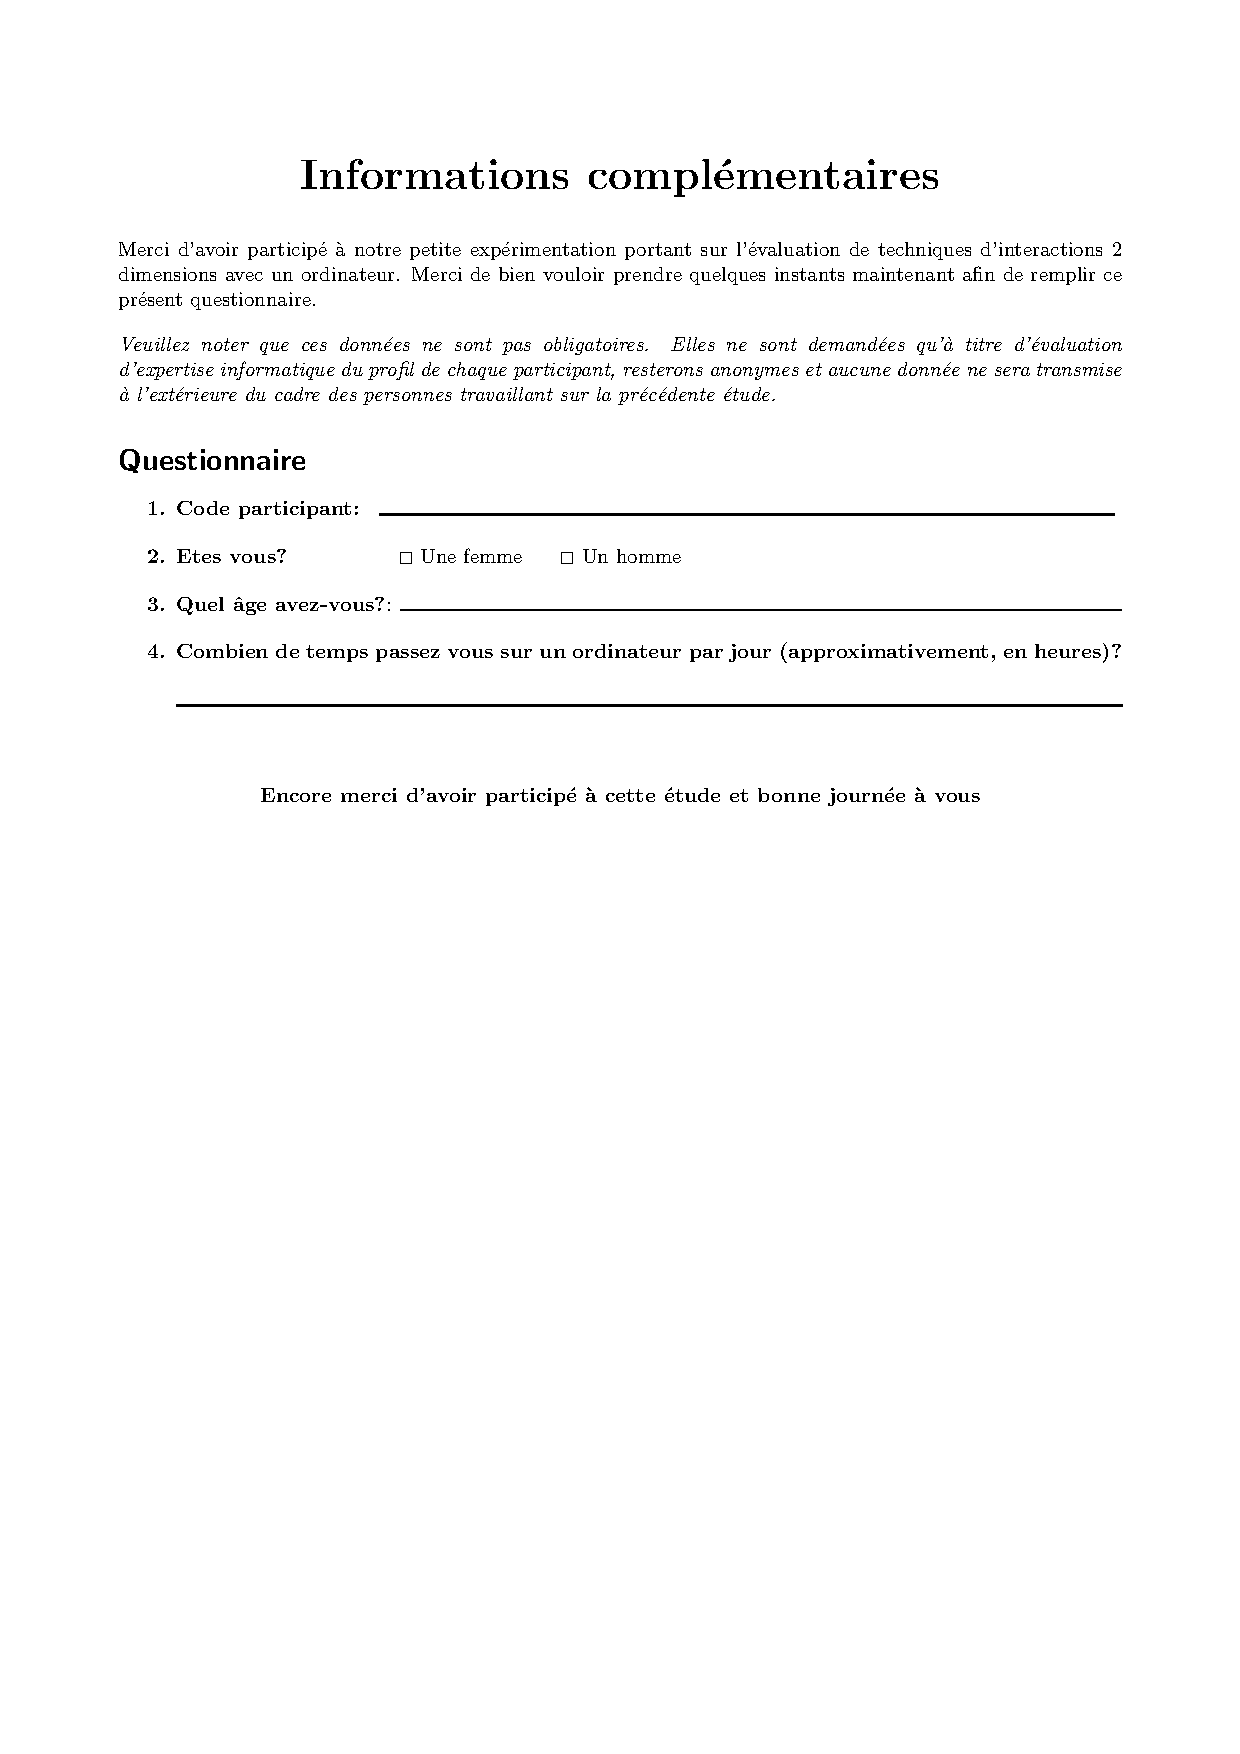
\includepdf[offset=70 -200, pagecommand={
    \addcontentsline{toc}{subsection}{Annexes - Questionnaire à fournir}
    \subsection*{Annexes - Questionnaire à fournir} \label{asking}
}]{documents/questionnaire.pdf}

%%%%%%%%%%%%%%%%%%%%%%%%%%%
%%  END OF THE DOCUMENT  %%
%%%%%%%%%%%%%%%%%%%%%%%%%%%
\end{document}